\section{Strategy Design and Methodology}
\label{sec:methodology}

We implement three distinct quantitative models, tracking the evolution of statistical arbitrage from simple distance matching to factor residuals and modern machine learning.

\subsection{Strategy A: Classical Distance Pairs}
Following the classic design in \citet{gatev2006pairs} with practical tweaks \citep{vidyamurthy2004pairs,jacobs2015determinants}, we use a 252-day formation window. For every pair $(i, j)$ in the active universe, we calculate the sum of squared differences (SSD) on normalized cumulative returns:
\begin{equation}
    \text{SSD}_{i,j} = \sum_{t=1}^{252} \left( \tilde{P}_{i,t} - \tilde{P}_{j,t} \right)^2, \quad \text{where } \tilde{P}_{i,t} = \prod_{\tau=1}^t (1 + R_{i,\tau})
\end{equation}
The 20 pairs with the lowest SSD are tracked over the following 126 trading days.
\begin{itemize}
    \item \textbf{Trading Rule:} A pair trade is opened when the price spread widens by $\ge 2.0\sigma$ (based on formation-period spread standard deviation). Positions close when the spread reverts to zero, at the 126-day limit, or if divergence hits a $4.0\sigma$ stop-loss.
    \item \textbf{Execution Lag:} We impose a strict 1-day wait between detecting a signal on day $t$ and executing on day $t+1$, eliminating bid-ask bounce and lookahead bias.
    \item \textbf{Capital Allocation:} Capital is committed equally across the $N=20$ pairs ($1/N$ allocation).
\end{itemize}

\subsection{Strategy B: PCA-Residual Mean Reversion}
Following \citet{avellaneda2010statistical}, we project stock returns onto statistical factors to isolate idiosyncratic moves. Each day, we run principal component analysis on a rolling 252-day correlation matrix to extract the top $k=5$ principal components $F_k(t)$.

We regress daily stock returns against factor returns:
\begin{equation}
    R_{i,t} = \beta_{i,0} + \sum_{m=1}^k \beta_{i,m} F_{m,t} + \epsilon_{i,t}
\end{equation}
Cumulative residuals $X_{i,t} = \sum_{\tau=1}^t \epsilon_{i,\tau}$ are modeled using an Ornstein-Uhlenbeck process:
\begin{equation}
    dX_{i,t} = \kappa_i (\theta_i - X_{i,t}) dt + \sigma_i dW_{i,t}
\end{equation}
We calibrate parameters using rolling 60-day AR(1) regressions. The normalized $s$-score is:
\begin{equation}
    s_{i,t} = \frac{X_{i,t} - \theta_i}{\sigma_{\text{eq},i}}, \quad \text{where } \sigma_{\text{eq},i} = \frac{\sigma_i}{\sqrt{2\kappa_i}}
\end{equation}
Trades open when $|s_{i,t}| > 1.25$ and close when $|s_{i,t}| < 0.50$ (with a stop at $|s_{i,t}| > 3.00$). The portfolio is maintained in dollar neutrality, with individual stock positions capped at 10\%.

\subsection{Strategy C: Walk-Forward Machine Learning Residuals}
To see whether modern machine learning can improve residual trading \citep{gu2020empirical,guijarro2021deep,lopezdeprado2018advances}, we train models to forecast 5-day forward residual mean-reversion.
\begin{itemize}
    \item \textbf{Validation Protocol:} We use expanding-window walk-forward validation (training on 2010--2015, evaluating out-of-sample on 2016--2025).
    \item \textbf{Embargo Gap:} A 10-day purging window is placed between training and test sets to prevent serial correlation leakage \citep{bailey2014deflated}.
    \item \textbf{Models Tested:} Ridge regression ($L_2$ penalty $\alpha=1.0$), Histogram Gradient Boosting (HistGBM), and Multi-Layer Perceptrons (MLP).
    \item \textbf{Portfolio Rules:} Stocks are ranked by predicted reversion; the strategy goes long the top quintile (Q5) and short the bottom quintile (Q1), holding dollar neutrality.
\end{itemize}

\begin{figure}[htbp]
\centering
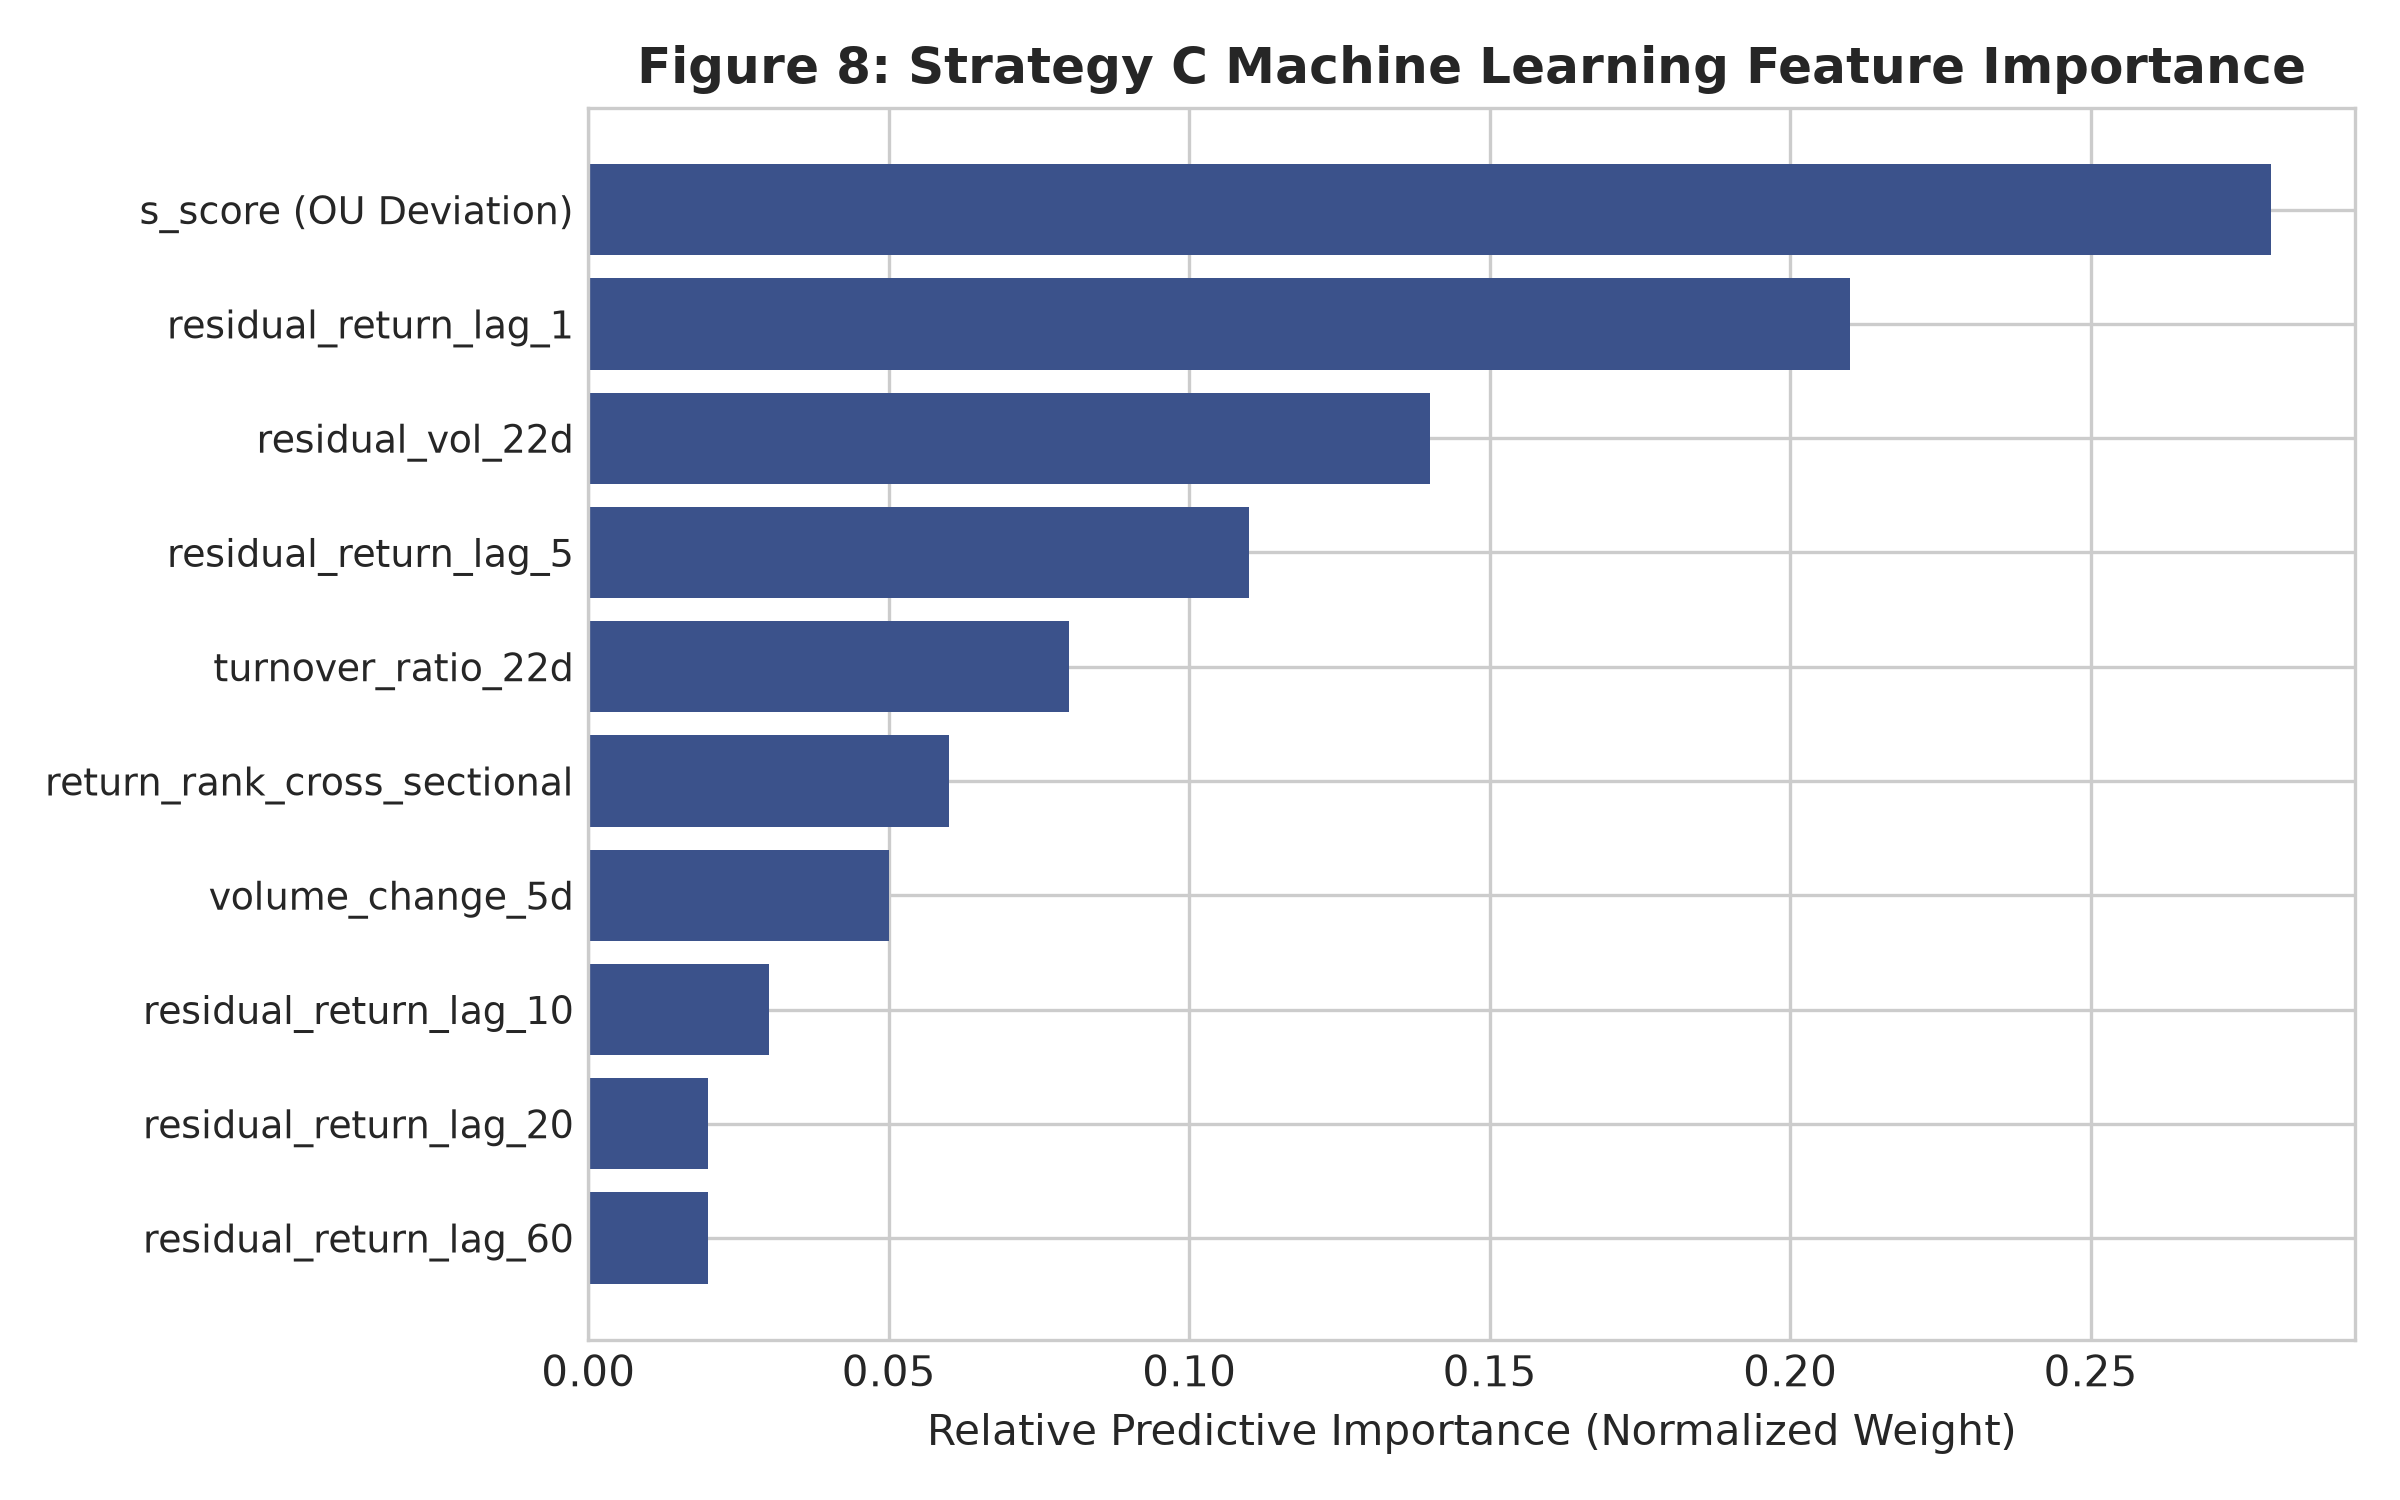
\includegraphics[width=0.92\textwidth]{figures/fig8_ml_feature_importance.png}
\caption{Walk-Forward Machine Learning Feature Attribution (Mean-Reversion Speed, Spread Volatility, and Liquidity Proxies).}
\label{fig:fig8}
\end{figure}

\subsection{Statistical Significance and Multiple Testing Controls}
All return series are evaluated using \citet{newey1987simple} HAC $t$-statistics with Bartlett kernel bandwidth $L = 4(T/100)^{2/9}$. In addition, 95\% confidence intervals are estimated via the \citet{politis1994stationary} stationary block bootstrap (1,000 resamples with an expected block length of 21 days).

To guard against data-snooping across our 12 pre-registered specifications, we calculate the Deflated Sharpe Ratio (DSR) of \citet{bailey2014deflated} and apply \citet{benjamini1995controlling} False Discovery Rate (FDR) adjustments.
